\section{Offset-Abgleich}
In dieser Teilaufgabe soll ein Offset-Abgleich (U$_a$ < 0,2~$mV$) durchgef\"uhrt werden.
\subsection{Experimentelle Durchf\"urung}
Der Operationsverst\"arker wird wie in Abbildung 6 aufgebaut. Zun\"achst wird die Offsetspannung am Ausgang ohne Offse Abgleich gemessen. Im zweiten Schritt wird ein Offset Abgleich durchgef\"urt, um die Offsetspannung unter 0.2~$mV$ zu reduzieren. F\"ur die Widerst\"ande wurden folgende Werte genommen: 
\begin{eqnarray*}
R_1 &=& 10~k\Omega\\
R_2 &=& 2,4~k\Omega\\
R_3 &=& 2~k\Omega\\
R_x &=& 22~k\Omega\\
R_z &=& 100~k\Omega
\end{eqnarray*}
F\"ur den Widerstand R$_y$ wurde f\"ur den Offset-Abgleich ein Potentiometer eingesetzt. 
\begin{figure}[!ht]
\begin{center}
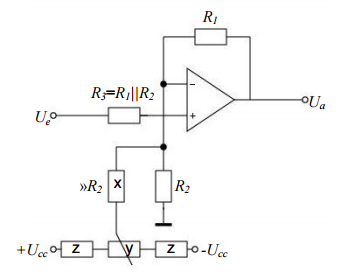
\includegraphics[scale=0.8]{bild/Schaltung}
\caption{Offsetkompensation f\"ur nichtinvertierenden OPV}
\end{center}
\end{figure}
\newpage
\subsection{Ergebnisse und Diskussion}
Die Offsetspannung ohne Offset Abgleich betrug 14,31~$mV$. Um diese Offsetspannung zu minimieren, wurde das Potentiometer auf ca. 20~$k\Omega$ eingesetzt. Durch das Einstellen des Potentiometers sank die Offsetspannung auf ca. 0.17~$mV$.


